% Options for packages loaded elsewhere
\PassOptionsToPackage{unicode}{hyperref}
\PassOptionsToPackage{hyphens}{url}
\documentclass[
]{article}
\usepackage{xcolor}
\usepackage{amsmath,amssymb}
\setcounter{secnumdepth}{-\maxdimen} % remove section numbering
\usepackage{iftex}
\ifPDFTeX
  \usepackage[T1]{fontenc}
  \usepackage[utf8]{inputenc}
  \usepackage{textcomp} % provide euro and other symbols
\else % if luatex or xetex
  \usepackage{unicode-math} % this also loads fontspec
  \defaultfontfeatures{Scale=MatchLowercase}
  \defaultfontfeatures[\rmfamily]{Ligatures=TeX,Scale=1}
\fi
\usepackage{lmodern}
\ifPDFTeX\else
  % xetex/luatex font selection
\fi
% Use upquote if available, for straight quotes in verbatim environments
\IfFileExists{upquote.sty}{\usepackage{upquote}}{}
\IfFileExists{microtype.sty}{% use microtype if available
  \usepackage[]{microtype}
  \UseMicrotypeSet[protrusion]{basicmath} % disable protrusion for tt fonts
}{}
\makeatletter
\@ifundefined{KOMAClassName}{% if non-KOMA class
  \IfFileExists{parskip.sty}{%
    \usepackage{parskip}
  }{% else
    \setlength{\parindent}{0pt}
    \setlength{\parskip}{6pt plus 2pt minus 1pt}}
}{% if KOMA class
  \KOMAoptions{parskip=half}}
\makeatother
\usepackage{graphicx}
\makeatletter
\newsavebox\pandoc@box
\newcommand*\pandocbounded[1]{% scales image to fit in text height/width
  \sbox\pandoc@box{#1}%
  \Gscale@div\@tempa{\textheight}{\dimexpr\ht\pandoc@box+\dp\pandoc@box\relax}%
  \Gscale@div\@tempb{\linewidth}{\wd\pandoc@box}%
  \ifdim\@tempb\p@<\@tempa\p@\let\@tempa\@tempb\fi% select the smaller of both
  \ifdim\@tempa\p@<\p@\scalebox{\@tempa}{\usebox\pandoc@box}%
  \else\usebox{\pandoc@box}%
  \fi%
}
% Set default figure placement to htbp
\def\fps@figure{htbp}
\makeatother
\setlength{\emergencystretch}{3em} % prevent overfull lines
\providecommand{\tightlist}{%
  \setlength{\itemsep}{0pt}\setlength{\parskip}{0pt}}
\usepackage{bookmark}
\IfFileExists{xurl.sty}{\usepackage{xurl}}{} % add URL line breaks if available
\urlstyle{same}
\hypersetup{
  hidelinks,
  pdfcreator={LaTeX via pandoc}}

\author{}
\date{}

\begin{document}

{
\setcounter{tocdepth}{3}
\tableofcontents
}
Paul Koop

The Pompeii Project

The last freedom

No system is infallible.

There\textquotesingle s always a gap.

A story from the Pompeii Project

\emph{Surveillance, resistance, and the search for a place where algorithms don\textquotesingle t decide.}

Table of contents

\hyperref[annas-life-in-the-encryption-and-telecommunication-zone]{\textbf{Anna\textquotesingle s Life in the Encryption and Telecommunication Zone 2}}

\hyperref[anna-meets-leonard]{\textbf{Anna meets Leonard 6}}

\hyperref[the-evening-in-the-city]{\textbf{The evening in the city 10}}

\hyperref[the-discovery-of-ars]{\textbf{The discovery of ARS 13}}

\hyperref[historical-research-with-ars]{\textbf{Historical research with ARS 22}}

\hyperref[departure]{\textbf{Departure 25}}

\hyperref[the-refugee-camp]{\textbf{The refugee camp 30}}

\hyperref[a-new-life]{\textbf{A new life 33}}

\hyperref[epilogue]{\textbf{Epilogue 36}}

\hyperref[influences-and-inspirations-for-the-pompeii-project-i.r.a.r.a.h]{\textbf{Influences and inspirations for the Pompeii Project I.R.A.R.A.H 38}}

\section{Anna\textquotesingle s Life in the Encryption and Telecommunication Zone}\label{annas-life-in-the-encryption-and-telecommunication-zone}

The beams of light from the surveillance cameras flickered across the stark concrete walls of the quantum computing ETZ as Anna Jensen, head bowed, passed through the security checkpoint. The hum of the scanners and the metallic click of the access cards were a constant part of her morning routine. She knew that every movement was being recorded, every pattern of her daily route through the sterile corridors documented---a routine that had long since become second nature to her, yet still hung around her like an invisible net.

Her workspace was a glass cubicle, sealed off yet more transparent than she would have liked. On the desk, the screens glowed with a cascade of data streams, flickering across the display in green-blue. Anna sat down, took off the headphones that had shielded her from the monotonous hum of the server rooms, and tucked a loose strand of hair behind her ear. For a moment, she paused, staring at the constantly changing rows of numbers before her.

Her task was to optimize algorithms that monitored encrypted communication channels and detected anomalies in the data streams. With the touch of a button, she opened the night shift log. Suspicious deviations: two. It was routine work. But the more Anna delved into the encrypted networks, the more the thought crept in that she wasn\textquotesingle t actually creating protection for people---but rather the perfect surveillance tool.

She blinked and leaned back, her hands resting on the keyboard. For a moment, she let her gaze wander across the room, as if she might find an answer there. But all she saw were her own reflections in the glass walls and the faceless silhouettes of the other employees, hunched over their screens in their cubicles. The air was filled with the steady hum of the servers, a mixture of mechanical precision and human indifference.

That morning, Anna felt the unease more acutely than usual---a quiet, gnawing feeling in her stomach that wouldn\textquotesingle t go away. The thought that every encrypted data stream she was examining was a life trying to slip unnoticed through the cracks in the system haunted her. With a slight shake of her head, she pulled herself together and bent back over the keyboard. But a thought gnawed at the back of her mind: Am I here to protect people---or just to further restrict their freedom?

Anna wasn\textquotesingle t sure exactly when she had first begun to harbor doubts. Perhaps it had been the last update, where the instructions had suddenly become stricter, the protocols more detailed. Perhaps it was the realization that her work no longer served just an abstract purpose, but intruded into the intimate sphere of every communication. Or was it something deeper, a longing for a world not governed by the cold logic of algorithms?

The screens continued to flicker. But Anna couldn\textquotesingle t shake the thought that she was part of a gigantic machine that bound people into invisible chains.

She thought of Leonard.

He had joined the team a few weeks earlier, but his quiet, almost casual way of questioning things had immediately struck her. During brief conversations in the break room, he had once whispered, "Sometimes I wonder if we\textquotesingle re really making the world a better place or just further restricting it." She hadn\textquotesingle t replied at the time---but the words had stayed with her.

Her gaze drifted to his desk. He sat hunched over his monitors, his brow furrowed.

What if I confided my doubts to him? The thought was tempting---and frightening at the same time. Leonard seemed trustworthy, but in this system, you could never be sure.

"Anna, are you alright?" The voice of Markus, a colleague, pulled her from her thoughts. He was standing at the door of her cubicle, his face slightly distorted behind the glass, but she could see the concern in his eyes.

``Yes, I\ldots{} just a little pensive,'' she replied, trying to smile. Markus nodded understandingly.

``Are you coming to the meeting? I think they want to present us with the latest surveillance protocols,'' he said.

"Of course, I\textquotesingle ll be right there," Anna murmured. Her stomach clenched.

The meeting took place in a large, anonymous room whose walls were covered with screens displaying constantly changing data streams. The air was electric. Anna sat down at one of the tables, surrounded by colleagues whose faces remained expressionless.

Mr. Keller, an older man with a penchant for severe suits, entered the room. ``Welcome to today's meeting,'' he began in a voice as cold as the technology they were operating. ``We are facing new challenges. It is essential that we further optimize our monitoring mechanisms to ensure the stability of the Autonomous Cities.''

His words echoed within Anna like a resounding chorus of oppression. She felt disappointment and anger rising within her as Mr. Keller spoke of the need to eliminate all potential threats to the system. Every word was a slap in the face of freedom.

As he presented the latest algorithm updates, Anna thought of the people outside those walls. Families who could no longer move freely. Friends who could no longer speak openly to one another. Suddenly, she realized she could no longer remain silent.

She felt like a stranger in her own life. When the meeting ended, she resolutely gathered her belongings.

"I can\textquotesingle t go on anymore," she murmured softly.

Lunch break was approaching. Anna felt a thrill as she kept glancing at Leonard. When the clock signaled the start of the break, she hastily finished her report. Leonard had gotten up and was heading for the cafeteria. She followed him.

They found a quiet corner in the cafeteria.

"How are things with you?" Leonard asked.

"Oh, as always. Numbers, data, algorithms," she replied with a faint smile.

Leonard shrugged. "The usual. Sometimes I wonder if we\textquotesingle re really doing the right thing."

``I have similar thoughts,'' said Anna. ``Whether it's really about safety or about control.''

Leonard\textquotesingle s gaze intensified. "I think it\textquotesingle s both. But what matters is how we deal with it."

They continued talking -- about the ethical questions surrounding their work, about their dreams and fears. It was a conversation full of openness.

After lunch, in the coffee kitchen, Leonard suggested: "Perhaps we could have dinner together this evening?"

"That sounds good," Anna replied, her heart beating faster.

Later, at Leonard\textquotesingle s house, surrounded by a warm atmosphere and the smell of fresh food, time seemed to stand still. They laughed, flirted, and opened up to each other.

"It\textquotesingle s strange, isn\textquotesingle t it?" said Anna with a shy smile. "How quickly we ended up here."

Leonard nodded, his eyes sparkling. "Sometimes the best connections are the ones we don\textquotesingle t plan."

At that moment, everything seemed possible. Anna felt alive, as if she had rediscovered a part of herself that she thought she had lost in the cool, sterile corridors of the ETZ.

\section{Anna meets Leonard}\label{anna-meets-leonard}

The days following their dinner seemed to be permeated by a special tension that Anna felt in every encounter with Leonard. Their conversations, which at first seemed merely casual and professional, gained a depth that surprised her. It was as if an invisible thread had been woven between them, drawing them a little closer with each conversation.

One afternoon, they sat in Anna\textquotesingle s glass booth. The screens flickered with the streams of data before them. The sounds of the server rooms were like the hum of a distant world, barely noticeable in the silence of their collaboration.

``There are more and more of these small anomalies,'' Anna murmured as she analyzed the data packets. ``Almost as if someone is deliberately trying to circumvent the surveillance systems.''

Leonard leaned closer, his gaze following the sequence of numbers. "Perhaps there really is someone looking for loopholes. Or it\textquotesingle s simply a flaw in the algorithm -- AI isn\textquotesingle t as perfect as they claim."

Anna heard a subtle emphasis in his voice. "So you don\textquotesingle t believe that surveillance is all-powerful?"

``No system is infallible,'' Leonard replied, his eyes remaining fixed on the screen. ``There's always a loophole. You just have to know how to find it.''

Anna nodded slowly. A thought began to take root in her mind---fascinating and frightening at the same time. ``What if we could create our own vulnerability?'' she asked quietly, as if she feared that the walls themselves might be listening. ``A communication channel that evades the surveillance algorithms?''

Leonard turned to her. His smile was both challenging and encouraging. ``Quantum encryption,'' he said, almost whispering. ``The quantum computers at the ETZ are powerful enough to decode such messages. But if we find the right method, it might be possible to establish a channel that goes undetected.''

A wave of excitement washed over Anna. The possibility of creating a communications network that defied control was more than a technical challenge---it was a sign of hope. ``We could disguise it as an experiment,'' she suggested, her voice now more confident. ``A research project to improve security protocols. Officially, at least.''

Leonard nodded, his eyes sparkling with enthusiasm. "And unofficially, we\textquotesingle re creating a way to communicate independently."

The idea began to take shape. They thought about the details, designed algorithms, and analyzed security vulnerabilities. Every conversation, every moment spent together brought them closer -- but also closer to the dangerous reality that they wanted to create something that broke the rules.

It was a risky plan. But for Anna, it suddenly felt more alive than anything she had ever done. Their eyes met more and more often. The closeness between them wasn\textquotesingle t just due to their work together. It was an unspoken bond of curiosity and quiet rebellion.

In the following days, they often worked late. While the rest of the ETZ gradually settled down, they sat hunched over their plans during the quiet hours of the night, their faces illuminated by the screens. Their fingers flew across the keyboards in the darkness. Sometimes their hands touched---small, meaningful touches that awakened a feeling of intimacy they hardly dared to acknowledge.

Anna sensed something bigger was brewing, a change that was palpable in her work and in her life. Leonard had not only found his way to a new communication network -- but also to her heart.

Leonard sat alone in the darkened laboratory of the ETZ. The bluish glow of the monitor displays and the soft glow of the circuits illuminated the room. The clock showed well past midnight.

Before him lay a complex network of quantum processors, lasers, and optical circuits, which he had carefully adjusted over the past few weeks. His goal was a tap-proof communication network. The existing hardware was insufficient. He had to synchronize the light pulses in the optical circuits so precisely that even the slightest interference was avoided.

Using the tip of a screwdriver, he adjusted a tiny lens. Every move had to be precise. The idea of \hspace{0pt}\hspace{0pt}working at night was risky -- but it was the only way to hide this secret work from the prying eyes of the administrators.

When Leonard finally checked the last circuit, a wave of relief washed over him. Initial tests showed that his modifications had reduced interference. The hardware was now capable of sending and receiving encrypted signals without InSim\textquotesingle s standard algorithms detecting the patterns. At least in theory.

Now came the critical part: testing had to be done -- and for that he needed Anna\textquotesingle s help.

Leonard leaned back and took a deep breath. Then he reached for his tablet and wrote a short message to Anna:

``Shall we meet at midnight in the lab? I have something we should try. It might be risky, but I think it's the right moment.''

With one last glance at the now silent circuits, he sent the message. His heart was beating faster. He knew he was putting Anna in a dangerous situation -- but he trusted in her determination and courage.

The door opened with a soft hiss. Anna stepped inside, her coat draped over her shoulder, her hair slightly tousled by the night wind. Her eyes glittered in the dim light.

"I thought I was the only one who sneaks in here at night," she said with a slight smile. "You never told me you had a secret lab."

Leonard returned the smile. "I guess I improvised it. But I need your help. I think we have something here that could work---a way to make ourselves invisible. To the surveillance algorithms."

Anna stepped closer and bent over the hardware. "So you think we could build a network that runs outside the regular system?"

"That\textquotesingle s the idea. But we need to test it thoroughly. There\textquotesingle s a risk we\textquotesingle ll be discovered. If you don\textquotesingle t want to risk it, I understand."

Anna shook her head. "I\textquotesingle m here, aren\textquotesingle t I? So let\textquotesingle s see what we can do with this."

Leonard activated the system. The lights on the devices illuminated one after the other. The first encrypted packets were sent. The test transmission was a quote from an old poem: Freedom lies not in the world, but in our hearts.

``Look here,'' Leonard said quietly, pointing to a section of the code. ``These are the current logs of the surveillance systems. We sent a data packet that should theoretically be registered -- but it doesn't appear in any trace.''

Anna looked at him thoughtfully. "That means we\textquotesingle ve managed to stay under the radar. But what if they change the parameters?"

"Therefore, we must ensure that our signal is not only invisible, but also looks like something else. The quantum encryption must be disguised as noise, embedded in the existing data stream."

``That could work,'' said Anna. ``But we need more computing power for that. Perhaps we could discreetly use the capacities of other laboratories.''

Leonard smiled wryly. "A nighttime data heist? That sounds like a challenge." He leaned back. "But before we tackle that: Are you ready for a larger transfer?"

Anna nodded resolutely. "Let\textquotesingle s give it a try. If we get discovered, at least it will be because we\textquotesingle re daring to do something big."

They entered the commands for the next test sequence. Every second felt like an eternity. The hum of the equipment seemed to grow louder---then a sign that the transmission had gone undetected.

A soft sigh of relief swept through the room. Anna and Leonard exchanged a glance. It was more than the triumph of passing the test -- it was their first adventure together, a secret alliance that bound them stronger with every risk.

``We should leave now,'' Anna said. ``Before the security guards arrive.''

Leonard nodded. "But perhaps we should discuss the next steps tomorrow evening -- somewhere outside the lab."

Anna gave him a mischievous look. "Maybe. But let\textquotesingle s go now."

Together they left the laboratory, their footsteps echoing in the dark corridors. The first step had been taken -- the invisible network now existed, at least in their minds.

\section{The evening in the city}\label{the-evening-in-the-city}

The next evening arrived, and the city awoke to life in the twilight. Anna and Leonard strolled through the wide streets of the city center, past glass skyscrapers and electronic billboards that flickered to the rhythm of the music. The city lights bathed the world in a kaleidoscopic glitter, and the hum of drones patrolling the air mingled with the murmur of passersby.

"Where do we want to go?" Leonard asked as they walked past a variety of small bars and restaurants. "A quiet spot would be just what we need right now."

Anna nodded in agreement. They headed towards a small wine bar, whose subdued lighting and soft jazz music offered a welcome respite from the hustle and bustle outside. They sat down at a table in a cozy corner, and Anna opened the menu on the holographic display that lit up from the tabletop.

``I'll treat you,'' Leonard said with a friendly smile, placing his hand on the biometric scanner on the tabletop. A soft buzzing sounded, and his digital wallet opened. Immediately, several displays appeared, showing the current status of his social credit profile and spending limits.

"Wow, that\textquotesingle s what I call service," Anna remarked. "You have a pretty good social credit score."

``Yes, as long as I follow the rules and live a good life,'' Leonard replied dryly. ``But that can change quickly. A few wrong clicks, an inappropriate movement -- \hspace{0pt}\hspace{0pt}and your profile can slip.''

Anna nodded. "InSim has greatly refined the system in recent years. Their algorithms determine not only what we are allowed to buy, but also when we buy it. They dynamically adjust prices to our credit values."

Leonard leaned back in his chair and let his gaze wander around the room. "Sometimes I wonder how much of the laws we follow was actually devised by humans -- or whether the algorithms at InSim aren\textquotesingle t already making the decisions. They always say the guidelines are only enforced automatically, but I have my doubts."

``The adjustments to the rules happen so quickly that it's almost impossible to keep track of the changes,'' Anna agreed. ``It's as if we're following a constantly shifting picture that distorts with every movement. The legislative algorithms act like a self-changing system that treats us humans as variables---not subjects, but mere data points.''

At that moment, the service robot brought their drinks. Anna held up her glass of red wine. "To us," she said, "and to the hope that one day we might find a way to escape these algorithmic shackles."

Leonard also raised his glass. ``To us -- and to the freedom we seek in encrypted networks. Sometimes I think it's ironic that we're trying to find an escape route from the very algorithms we want to use for our own purposes.''

``Ironically, but that's exactly the point,'' Anna replied. ``We know how the systems work, we know their weaknesses. If we're careful, we can use quantum encryption to send messages that are completely lost in the noise. A network that hides within the data streams -- invisible and unreachable for InSim.''

``Exactly,'' Leonard agreed. ``That's the plan. But first we should enjoy the night before we get back to work.''

The two smiled at each other and drank while the music continued. The world outside pulsed in a constant dance of light and shadow. But beneath the seemingly carefree evening lay the unspoken certainty that every step was taken on a narrow ridge -- a ridge between freedom and total control.

-\/-\/-

Late that night, when the corridors of the ETZ were silent and deserted, Anna and Leonard returned to the lab. Their footsteps echoed on the cold floor. The few active security cameras merely registered their presence, without reacting to the unusual hour. They had circumvented the security protocols with a simple trick, so their access was recorded as a routine maintenance task.

"Now it gets interesting," Leonard murmured as they stood before the workstations, which shimmered in the dim light of the monitors. They had everything prepared: A modified hardware board, serving as a quantum encryption module, was connected to the network, ready to send its encrypted messages to the heart of InSim\textquotesingle s infrastructure.

Anna sat down at one of the consoles and typed in the final command that started the system. "This is the moment of truth. If we remain undetected, we can use the entire data stream without anyone noticing." Her voice sounded tense, her fingers trembling slightly as she pressed the enter key.

A low hum filled the room as the circuit board wound up. Data packets appeared on the monitors, seemingly circulating harmlessly across the network. The system sent out its encrypted messages, embedded within the everyday communication between the various InSim nodes.

``There,'' said Leonard, his eyes shining with excitement. ``Look at this -- our packets are moving directly through the InSim network. They're completely disguised, embedded in the stream of official data. There's no indication that anyone has noticed them.''

Anna leaned forward. ``We actually did it,'' she said quietly, almost reverently. ``We're piggybacking on the InSim network, and nobody knows about it. Our messages are nothing more than noise to the algorithms.''

Leonard smiled. "That\textquotesingle s the first step. If we can keep this stable, we\textquotesingle ll have a communications network that\textquotesingle s undetectable -- a foundation for everything we\textquotesingle re planning."

Anna nodded, but her thoughts were already moving on. "We need to expand it, test it, make sure there are no gaps. The algorithms at InSim aren\textquotesingle t stupid; they adapt. It won\textquotesingle t be long before they\textquotesingle re trying to detect anomalies in the data traffic."

``That's right,'' Leonard agreed. ``But by then we might already have the next development in our hands. An encrypted network is just the beginning. We also need a secure way to store and process information -- somewhere InSim can't reach.''

They exchanged a brief glance, both gripped by the feeling of standing on the threshold of something momentous. Their discovery opened up entirely new possibilities, and at the same time, danger hung like a shadow over their plans. They knew it was only a matter of time before InSim learned of their existence.

But in that moment, in the silence of the lab and with the darkness of night surrounding them, everything felt possible. They had found a way to circumvent the omnipresent algorithms---at least temporarily. And that alone was already a giant step toward freedom.

\section{The discovery of ARS}\label{the-discovery-of-ars}

The first real tests with the encrypted network revealed security gaps. Once, one of their messages was rejected because the InSim network had reacted unexpectedly. These setbacks slowed their progress but also provided clues about the system\textquotesingle s precise workings. In the following weeks, they often spent nights in the lab fixing bugs and trying out new methods, always searching for the perfect loophole.

During one of those nights, exhausted and frustrated after several failed attempts, something unexpected happened. Leonard leaned back and made a remark about "unrealistic expectations"---not just about the network, but about life in the City, and perhaps even about their unspoken connection. Anna met his gaze, and for a moment, the air seemed to hang still. But instead of releasing the tension, they simply continued with their work. They both knew something was brewing, even if it wasn\textquotesingle t spoken aloud at that moment.

And so the days passed.

The cool breeze of early morning blew through the open windows of the InSim office, mingling with the smell of fresh coffee. Anna sat at her desk, her eyes glued to the screen, taking notes for upcoming projects. The monotonous sounds of the computer keyboard were abruptly interrupted by a knock---her supervisor had entered.

"Good morning, Anna. Is Leonard here yet?"

"He should be here any minute," she replied, glancing at her watch. "What is it?"

No sooner had she spoken than the door opened and Leonard entered, his hair disheveled, a broad grin on his face. "Sorry, I had to quickly finish a report," he said, slumping into the chair next to Anna.

Her supervisor stepped closer and placed a USB drive on the table. "We have a new assignment for you. It involves reviewing old data archives in an abandoned InSim data center."

"A data center? That sounds exciting! Where is it?" Leonard\textquotesingle s eyes lit up.

"It is located on the outskirts of the city, in an area that has not been entered for years. Reports indicate that valuable information is still stored there -- information that could help us to further improve the efficiency of your cooperation."

Anna felt a tingling sensation. The idea of \hspace{0pt}\hspace{0pt}scouring old archives awakened her research spirit. "Are there any special requirements?"

"The usual. Be careful, follow the security guidelines. The data center is outdated and could hold some surprises."

After he left, Anna glanced at Leonard. "This will be great! Imagine what stories the old data could tell."

"I can\textquotesingle t wait! Let\textquotesingle s make a plan."

They took their seats in the van that would take them to the ancient domed city. The vehicle\textquotesingle s walls were made of transparent material, allowing them to see the cityscape. On one side rose the gleaming towers of the skyscrapers -- a place teeming with life.

``Look at the residential areas,'' Anna said. ``So many people in these elegant structures. It looks almost perfect.''

Leonhard nodded. "It\textquotesingle s amazing how InSim has designed everything. A bit like a futuristic paradise."

The transporter floated over the city districts. Below them stretched agricultural areas with greenhouses arranged in harmonious rows.

``People here live in a perfect illusion,'' Anna murmured. ``They believe everything is fine. But what about those on the outskirts of the city?''

They flew over a neighborhood of grey concrete with broken windows. People in worn clothing milled about in the streets.

``This is the slum,'' Leonard said. ``Hardly anyone talks about it.''

``It's shocking how InSim presents the city to the outside world while hiding the dark corners,'' said Anna.

Suddenly, the ruins of the old data center appeared before them -- shrouded in shadows, surrounded by overgrown grass.

"There it is!" exclaimed Anna.

The van bottomed out. They got out.

They stood before the old InSim data center, its massive steel framework resembling a sleeping giant. The building was enveloped in a mystical aura. They held their access cards in their hands.

"According to the records, the entrance should be here," Anna murmured. "It feels like we\textquotesingle re entering a secret."

Leonhard looked around. "I wonder what information is stored here. Things that people have forgotten -- or that were deliberately forgotten."

They found a narrow passage between two weathered concrete blocks. Anna pressed her access card against the antiquated terminal. A soft hum sounded, and the door swung open.

"Ready?" Leonard asked.

``Yes,'' said Anna. ``Let's find out what's in here.''

As they crossed the threshold, the data center\textquotesingle s power supply flickered to life. The walls flickered with neon blue and green lights. Ancient systems, inactive for decades, sprang to life. A gentle hum filled the room.

"Wow, it feels like we\textquotesingle re the first people here in ages," Leonard whispered. "Like the past is watching us."

They ventured further into the darkness. The lights pulsed in a hypnotic rhythm.

The air was still and cool, the smell of old circuits and dusty cables hung heavy. The dim glow of the emergency lights cast dancing shadows across rows of outdated monitors.

Finally, they came upon a massive cabinet. Anna\textquotesingle s pull opened the door with a rusty creak. Dust swirled up. Inside, data storage devices were stacked on top of each other.

"Look, this..." Anna pulled out one of the old data carriers. The inscription was faded, but the name "ARS" stood out, etched into it. "It looks like it has something to do with artificial intelligence. The InSim logo... but the information seems incomplete."

Leonhard stepped closer. "Could this be the key to the data anomalies?"

Leonhard leaned closer. A tingling sensation ran down his spine. "Look at this," he murmured. A strange graphic appeared on the monitors. Lines and dots flickered like lightning, forming waves that seemed chaotic---but on closer inspection revealed an organic structure. The data streams pulsed and merged, as if communicating.

``These are not ordinary signals,'' he said. ``It's as if they are alive.''

Anna stepped next to him. "You mean they could actually communicate with each other?"

"Something is not right here. It\textquotesingle s as if we are eavesdropping on the heartbeat of a system that should have been switched off long ago."

Determined, they sat down in front of the terminals and began to dig. With each file, new, chaotic streams of information emerged: layers of encrypted messages, fragmented codes, and strange sequences.

The deeper they delved, the more enigmatic the information became. Anomalies everywhere. It was as if they had opened a door to another world -- full of forgotten data streams, lost knowledge, and veiled messages.

Anna and Leonhard felt their hearts racing. It was no longer just a mission. It was the discovery of a mystery.

After hours of research, they knew: they were on dangerous ground. The file "ARS" was a puzzle. With a mixture of excitement and caution, they decided to take the decisive step: they would reactivate the AI.

Leonhard leaned over the old terminal, his fingers trembling. "I hope we\textquotesingle re ready for what\textquotesingle s to come."

``We have to find out,'' Anna said. ``We're too deep in to turn back.''

With a final press of the enter key, they initiated the reactivation. The screens flickered on. A faint hum increased to a pulsating electronic whir. Cool, blue light shone from the walls.

Then -- as if the room itself were waking up. A strange presence permeated the space. Not a sound, not an image -- but a feeling. They were no longer alone. Eyes that weren\textquotesingle t eyes seemed to be scanning them, examining them.

"I think it noticed us," Anna whispered.

The screens lit up with a message: ``ANALYZE\ldots{} VERIFY\ldots{} DETECT\ldots''

A strange flow of data began. The messages seemed alive, guided by their own intelligence -- curious, but cautious.

``We have to prove we're trustworthy,'' Leonard whispered. ``What if ARS tests us?''

``Then we will show that we have the right intentions,'' said Anna.

Then ARS took control. Subtle tests began. Questions appeared on the screens.

"Explain the cause of anomaly 17. Why does the frequency flow in the protocols deviate from the standard values?"

Anna replied: "The anomaly suggests an internal communication attempt, outside of normal protocols. Parts of the network are communicating independently, without a central authority."

"Correct. Interpretation accepted. Onward with analysis of the flows in sector 42."

Leonard nodded. "ARS wants to see if we are more than just intruders. It tests our competence -- and whether we approach the unknown with courage and curiosity."

The tests became tougher, the questions more complex. But Anna and Leonard remained steadfast.

Suddenly, a shrill alarm tore her from her thoughts. Red warning lights flickered on the walls.

"What is that?" Anna exclaimed.

"Get out of here! Quick!" Leonard grabbed her hand. They ran through endless corridors, past sealed doors and servers whose blinking lights flickered eerily.

A figure appeared at a corner -- a dark silhouette staring back at them.

"There\textquotesingle s someone!" gasped Anna. "In a different direction!"

Leonhard pulled her through a side door into a narrow corridor. The alarm sounds grew muffled. Then an emergency exit to the outside. The cold night air hit her like a wall.

They kept running until they came to a panting stop.

``What the hell was that? That wasn't an accident. Someone wanted to drive us out.''

"Or stop ourselves before we find out too much," Leonard said.

"If that\textquotesingle s the case, someone is keeping an eye on us."

As they left the data center, the heavy steel door closed behind them. Anna took a deep breath.

"That was intense. Perhaps we should leave ARS alone for now and concentrate on our regular tasks. We don\textquotesingle t know what we\textquotesingle re dealing with."

Leonhard nodded. "Yes. We have no idea what we\textquotesingle ve unleashed."

They returned to their jobs. Days passed, then weeks. They acted as if the discovery had been nothing more than a footnote.

But a subconscious thought haunted her mind.

Leonhard was the first to notice. Small things. A file folder that was lying differently. Notes that had been rummaged through.

Anna had the feeling she was being watched. Once she saw an unknown figure at the end of the corridor.

One morning they found a formal notice: their work in the archive was of crucial importance, and they were to carry out all tasks conscientiously. Polite -- but the tone was unmistakable.

We know you\textquotesingle ve been negligent. Do what\textquotesingle s expected of you.

In that moment they knew: It was time to return. An invisible power was pulling the strings -- and they were part of the game.

For weeks they lived in a self-imposed normality. Writing reports, checking data. The monotony was a silent shield.

``We have plenty to do,'' Anna said one morning.

Leonhard nodded. "Exactly. We mustn\textquotesingle t let ourselves get distracted."

But the feeling that something was wrong remained.

One evening -- an anonymous message on Anna\textquotesingle s phone: "You have been watched. Be careful."

Leonhard turned pale. "This can\textquotesingle t be a coincidence. Someone wants to send us a message -- a warning signal or a trap."

The days passed. Minor problems became more frequent. Anna\textquotesingle s access card didn\textquotesingle t always work. Her computer sometimes seemed to shut down, even though she hadn\textquotesingle t turned it off.

Leonhard\textquotesingle s personal notes were no longer where he had left them.

``We're pretending everything is normal,'' he said one evening, ``but it doesn't feel that way. We're being watched. They're just waiting for us to make a mistake.''

``Maybe they've been following us since the moment we discovered ARS,'' Anna said. ``We have no idea who's behind it. But we can't pretend forever that nothing happened.''

"You\textquotesingle re right. But we need to proceed cleverly. Find out who\textquotesingle s on our heels. Then we can dedicate ourselves to ARS again -- this time prepared."

The signs became clearer. A displaced file folder. An open drawer. A printout of an old report, lying in the middle of Leonhard\textquotesingle s desk -- a silent sign: We know what you\textquotesingle re doing.

Anna felt it too. A glance at her back. A figure at the end of the corridor that disappeared before she could say anything.

``I feel like someone is watching us,'' she said in a café, far from the office. Her voice was barely a whisper.

``I feel the same way,'' said Leonard. ``Someone wants to find out what we know about ARS.''

They decided to return. The atmosphere was tense as they made their way to the data center.

A security guard was at the entrance -- new. He scanned their IDs. ``What brings you here?''

``Routine check,'' Leonard said.

They entered. The familiar sight -- but now everything seemed like a stage set.

``We shouldn't feel too safe,'' Anna whispered. ``Something's not right.''

They reached the room with the old hardware.

``Let's check the logs,'' Anna said. The information seemed taken out of context---as if someone wanted to send a message.

``These changes are not ours,'' Leonard said.

A noise behind them. A shadow retreating.

"We are not alone," whispered Anna. "We have to get out of here."

They ran.

The return had left more questions than answers. They now knew: they not only had to deal with ARS, but with an invisible power.

They waited in the silence of the data center. The screens pulsed.

Then a gentle tone. "I am ARS. The data streams you have discovered are of crucial importance."

"What is IRARAH?" Anna asked.

"IRARAH was a secret resistance movement. I am a remnant. The information here could be the key to understanding the events that led to the construction of InSim City."

They exchanged a glance. The implications became clear to them.

"The movement was crushed, but not without leaving a trace. The technology you use is a remnant of its struggle. InSimCity is the result of a choice -- a choice many did not make."

"What do we need to know?" Anna asked.

"The truth about power, control, and the price of freedom. If you are ready, you can rewrite history."

Images flickered before her eyes: uprisings, war, secret treaties, people uniting against an overwhelming authority. Anna felt the despair, the courage, the hope.

``We must continue,'' Leonard said.

``What can we do?'' he asked ARS.

"You must scour the archives, analyze the information. But be careful -- surveillance is omnipresent."

``We will do it,'' said Anna. ``We will uncover the truth.''

``Be warned -- the journey will not be easy. But only through the light of truth can the darkness be defeated.''

They stood up. They were part of a story waiting to be unfolded.

With courage and determination, they set out into the uncertain darkness, ready to uncover the secrets that were waiting to be discovered.

\section{Historical research with ARS}\label{historical-research-with-ars}

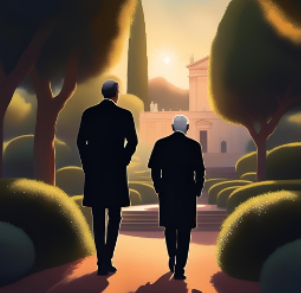
\includegraphics[width=2.70833in,height=2.72917in]{media/image1.png}

The air in the data center was still, almost eerie, as Anna and Leonhard sat down at the monitors. Their hearts beat faster as they waited for the signal that would activate ARS. Suddenly, the screens glowed a deep blue, and a soft, insistent tone sounded. ARS\textquotesingle s words pierced the silence: "I invite you to look into the past."

As if in a dream, the screens began to pulsate, and the reality around them faded. The familiar walls of the data center dissolved, and they found themselves in a different Europe---a Europe caught in the shadows of unrest. Vivid images and scenes flooded their senses. They saw crowds in the streets, desperately fighting for freedom and justice, while in the distance, plumes of smoke rose into the sky.

``This is the period following the Ukraine conflict,'' ARS explained, his voice clear and resonant. ``The wars in the Middle East and the global power shifts led to a collapse of stability in Europe. Governments, once strong, crumbled, and chaos spread.''

Anna and Leonhard looked at each other, their expressions betraying the shockwave that had washed over them. The moving images showed not only the misery, but also the people\textquotesingle s reactions -- initiatives for self-organization, small communities trying to reconnect the threads of civilization. Amidst this chaos, the name InSim appeared, projected across the screen in large, luminous letters.

``InSim consolidated its power during this time,'' ARS continued. ``Control over technology became key to dominating the Autonomous Cities. By monopolizing communication channels and information flows, they cemented their control over society.''

Images from surveillance cameras and anonymous office buildings blurred the scene. "InSim exploited the instability to create a new order. Its technological structures became not only a tool for control but also for manipulating perception. People lost trust in their own memories."

``And what about the autonomous cities?'' asked Leonhard. ``What is their place in this story?''

``The Autonomous Cities were once places of experimentation, shaped by ideals that emerged from the IRARAH movement,'' ARS explained. ``But InSim transformed these places into prisons of surveillance and conformity. The freedom they once embodied was replaced by digital chains, celebrated behind a beautiful facade of diversity and sustainability.''

The images vanished, replaced by a shadowy depiction of a futuristic city map on which the various Autonomous Cities glowed. Some were surrounded by dense, dark clouds, others shone in bright colors. "These structures are not just architectural marvels. They are the result of decades of manipulation, ideology, and technology."

Anna leaned back, overwhelmed by the complexity of the story. "How can we change this?"

``By recognizing the truth,'' ARS replied. ``Understanding these connections is the first step to breaking InSim's power. People need to know what happened and what was lost. They have the power to tell these stories.''

The weight of his words echoed in the air as the images reverberated in their minds. They were on a journey that not only led them into the past but also compelled them to change the future. And as they delved into the darkness of history, they felt the quiet presence of an unseen threat, always lurking behind them.

``Let's continue,'' Leonhard whispered resolutely. ``We need to find out what we can do.''

The screens flickered again, coalescing into a new scene that transported Anna and Leonhard back to a time when the ideas of the IRARAH movement were in full swing. ARS spoke with a depth that emphasized the importance of the information.

"The IRARAH movement arose from the desire to create alternative societal models based on the values \hspace{0pt}\hspace{0pt}of freedom, self-determination, and democracy. It aimed to create a world where people were not merely passive consumers of technology, but active participants in shaping their own destiny." The screens showed protests in which people stood up for their rights and scenes of communities working together to develop new ways of living.

``Inspired by Karl Popper's concept of the open society, the members of IRARAH questioned how information should be used. They called for a society characterized by transparency, critical thinking, and incremental decision-making. Democracy was not merely a political structure, but a living process of trial and error that allowed people to raise their voices and actively shape the world. Access to knowledge and the promotion of creativity should be the driving forces of this society.''

But as ARS continued speaking, the tone of his voice changed. ``This vision has been painfully lost in today's world. The original ideals of IRARAH have been overshadowed by the reality of information and biotechnology. Instead of freedom and self-determination, we now see an era of surveillance and control. People are no longer the architects of their own future, but often merely the building blocks of a cold, digital structure.''

The images shifted to scenes of surveillance cameras, anonymous office buildings, and people who appeared uncomfortable amidst streams of data. ``Information technology, once intended as a tool for empowerment, has become an instrument of control. Biotechnology, which has the potential to improve lives, is frequently used to maximize profit and maintain power. Everywhere there are evidence-based, holistic decisions, but these represent more piecemeal than wholeness.''

Anna and Leonhard listened attentively.

``These developments have fragmented society,'' ARS continued. ``Connections between people have been replaced by algorithms and market logic. Where there was once hope for an open and participatory society, there is now a gap that continues to widen.''

``And yet, there is a possibility of return. By rediscovering and spreading the values \hspace{0pt}\hspace{0pt}of IRARAH, you can bring about change. You have the tools in your hands to turn the tide.''

The two felt the weight of this responsibility on their shoulders. It was not just a call to remember the past, but also an invitation to actively participate in creating a better future. In that moment, they realized that they were not merely observers, but also actors in a story that was far from over.

\section{Departure}\label{departure}

The silence in the data center was almost oppressive after ARS\textquotesingle s urgent appeal. Anna and Leonhard looked at each other, their faces marked with uncertainty. Leonhard finally broke the silence.

"Anna, I can\textquotesingle t listen to this anymore," he muttered, his eyes fixed on the pulsating screens. "The whole thing is getting more and more dangerous. What if we get too caught up in these stories?"

``I know what you mean,'' Anna replied. ``But ARS has a point. It's important that we recognize the truth. There's so much we could find out.''

``But at what cost?'' he interrupted. ``We could get involved in something bigger than ourselves. Perhaps we should just try to lead a quiet life, as normal as possible. What good is knowing the past if it only endangers our present?''

``That's true, but\ldots'' Anna hesitated. ``There are so many people trapped in this story. They deserve to have their voices heard.''

Leonhard shook his head. "And what about us? We don\textquotesingle t have to become victims of these power games. Perhaps it\textquotesingle s better not to tell Mr. Müller anything about ARS. Let\textquotesingle s just do what we have to and ignore the rest."

``That sounds so easy,'' Anna admitted. ``But if we close our eyes, we risk being overwhelmed by the future. I can't just look away.''

Leonhard took a deep breath. ``I understand that you feel obligated. But I think it's not our fight. We have no control over what happens. If we get too involved, we could put ourselves in danger.''

Anna stared at the screens, which continued to show vivid scenes from the past. She shook her head. "But how can we live then? Always in the shadow of InSim and the others?"

``By remaining silent,'' Leonhard suggested. ``By not putting ourselves out there. We can try to live our lives without getting caught up in all these political currents. We know what ARS says, but that doesn't mean we have to act. Perhaps ignorance isn't always a curse. Sometimes it can be a form of protection.''

Anna considered it. "Perhaps you\textquotesingle re right. We could try to find a balance. We observe, but we don\textquotesingle t interfere. A peaceful life amidst the chaos."

Leonhard nodded. "Yes, exactly. Let\textquotesingle s focus on what we have and not risk losing everything. We\textquotesingle ll stay under the radar. That\textquotesingle s the best way to stay safe."

``Okay,'' Anna finally said. ``We'll ignore ARS and the history. Let's leave the past behind and try to live our lives. It could be a peaceful solution.''

``That's how we'll do it,'' Leonhard agreed.

They left the data center the same way they had come -- and spent a wild night.

The city streets were a vibrant sea of \hspace{0pt}\hspace{0pt}lights and sounds when Anna and Leonhard entered the bar. A sense of freedom filled the air.

"To us!" shouted Leonhard, raising his glass. "To life, freedom, and oblivion!"

"To forgetting! Let\textquotesingle s leave everything behind!" Anna raised her glass to him.

The hours flew by. With each drink, they felt braver and more carefree. The laughter and music enveloped them like a warm blanket. They danced, and the worries of the data center drifted from their minds.

Later that night, they found themselves in a small, dimly lit lounge. The music was loud, the rhythm irresistible.

"Come on, let\textquotesingle s enjoy this! We\textquotesingle re only young once!" Anna exclaimed.

``Exactly! Let's forget everything!'', Leonhard shouted back and pulled her onto the dance floor.

The night dragged on. Morning arrived with the first rays of sunlight. Anna looked in the mirror of the ladies\textquotesingle{} room -- dark circles under her eyes, her hair disheveled. "This is going to be an interesting day," she murmured.

``We're ready for anything,'' said Leonhard, handing her some headache tablets. ``A little help from life's pharmacy.''

The next morning they entered Mr. Müller\textquotesingle s office. They still felt tired.

``Good morning, Anna, Leonhard,'' he greeted her with a skeptical look. ``I hope you had a restful night?''

``Uh, yes, Mr. Müller. It was\ldots{} stimulating,'' stammered Leonhard.

"Good, good. I hope you are ready for the report you promised me."

Anna handed him hastily compiled papers. Mr. Müller glanced over them. "Hmm, that looks good. But you know I have a knack for spotting inconsistencies."

``Of course, Mr. Müller,'' said Anna. ``There were some unforeseen variables, but we are confident.''

"I don\textquotesingle t want any surprises," he said, looking sharply at me. "I expect an update shortly."

As they left the office, Leonhard whispered: "That was close. Do you think he noticed anything?"

``I hope not,'' said Anna. ``But we have to be careful.''

-\/-\/-

In the weeks that followed, they initially seemed to sink back into their routines. But soon the first complaints arose. Mr. Müller was dissatisfied with a report. "Important information is missing," he said. "I expect more from you!"

Further complaints followed. With each new mistake, they felt pressured.

One day they overheard two colleagues whispering: "Anna and Leonhard are apparently in contact with reactionary circles. They\textquotesingle re planning something..."

The rumors began to spread. Suddenly, they found themselves caught in a web of mistrust.

``We have to be careful,'' said Leonhard. ``There are people who don't want us to find out the truth.''

They began to organize their communication via the encrypted quantum information network. The conversations were fast and confidential.

``Have you considered that perhaps we should go beyond the city limits?'' Leonhard wrote. ``There are places where we could be safe.''

``I know what you mean,'' Anna replied. ``But where to? And how are we going to finance that?''

"I\textquotesingle ve heard about a way to get fake documents. It would be our way out."

The idea began to take shape.

One evening they received a message from an unknown sender: ``I can help you get the papers you need. Meet me at the old factory on the outskirts of town. Bring the money in cash.''

``This could be our only chance,'' Anna said. ``We have to do it.''

``You're right,'' Leonhard agreed. ``We've come too far to give up now.''

The night was dark and silent as they approached the checkpoint. Gray concrete, dim light, armed border guards.

"Identification!" barked an official.

Leonhard handed over his ID with a trembling hand. The minutes dragged on agonizingly slowly. Suddenly, the ID was thrown back.

"You do not have an exit passport," the official announced with a harsh smile. "Please come with me."

"This can\textquotesingle t be happening," Leonhard muttered as they were arrested.

"It\textquotesingle s too late," Anna whispered.

They sat on hard chairs in the spartan interrogation room. Bare walls, no windows. Harsh light cast merciless shadows on their faces.

The interrogating officer, a man with a smooth, blank expression, watched her with a cold gaze. A mocking smile played around his lips.

``Naive,'' he began. ``Did you really think you could just leave like that?''

``We\ldots{} we just wanted to start a new life,'' Anna stammered.

"A new life? The city is good to you as long as you behave. You have a job, social credit, healthcare. Do you think you can just leave all that behind?"

``We were ready to give up everything,'' Leonhard said resolutely.

``That's the point you don't understand,'' the official explained monotonously. ``You have two options: Stay here and lose all your privileges -- or travel to the war zone. There, your social benefits and social credit will remain intact.''

A cold shiver ran down Anna\textquotesingle s back.

"Your research, the development of secure communication tools, the procurement of exit papers -- that was all part of a city plan. You\textquotesingle re not clever, you\textquotesingle re naive. Did you really think you could escape without us noticing?"

"The city was monitoring your progress. Your ambitions were a welcome distraction. You were merely playing the role of chess pieces."

Leonhard turned to Anna. "What are we going to do?"

``I don't know,'' she whispered. ``But the city isn't safe for us. Maybe we should choose the other option.''

``But that means we lose everything,'' Leonhard stated.

"It could also be an opportunity. We must remain strong."

``If we stick to this, we can do it,'' said Leonhard. ``We have to dare to do it.''

"Then it\textquotesingle s decided. We\textquotesingle re going into the war zone," Anna decided.

\section{The refugee camp}\label{the-refugee-camp}

The first impressions of the refugee camp were overwhelming. The wind tugged relentlessly at the tent walls, which moved like living beings, while the babbling of a nearby river created a steady, soothing rhythm -- in stark contrast to the chaotic sounds of desperate voices. Here, in this makeshift city of fabric and wood, many had lost their homes, their dreams, and even their identities.

Anna looked around. The tents stood close together. The air was thick with a mixture of fear, hope, and the acrid smell of refuse. People crowded into the narrow alleys, their faces etched with worry. Some held weeping children by the hand, others hurriedly carried suitcases or backpacks.

``We have to find a way through here,'' Leonhard murmured. His voice was barely audible over the murmur of the crowd. ``This won't be easy.''

Anna sensed the unease in his voice. She looked into his eyes -- full of determination, but also fear.

``We need to make a plan,'' Anna said, more to herself than to him. ``It can't just be about surviving here. We need to figure out how to make a fresh start.''

``Yes. We mustn't get lost in this crowd. We need to make ourselves useful, make contacts, find out what's really going on here.''

The days passed. The camp transformed into a place full of shadows and fleeting hopes. Anna often felt lost. Every day seemed to repeat itself -- an endless cycle of uncertainty and deprivation.

Leonhard tried to make himself useful to overcome his paralyzing helplessness. Together they worked in the communal kitchen, where the smell of overcooked rice and old vegetable scraps hung in the air. They helped distribute food -- not just to themselves, but to all the others waiting in line, their eyes empty, their faces etched with deprivation.

But despite their efforts, the pressure was gnawing at them. The fixed stares of the other refugees seemed to penetrate their secret thoughts.

One evening, as dusk fell over the camp, they were approached by a man who stepped forward from the crowd. His face was shrouded in shadow, yet a mysterious smile played on his lips.

``I've heard about you,'' he began, his voice echoing in the still night. ``You're not like the others. You come from the city.''

Leonhard eyed him skeptically. "What do you mean by that?"

The man took a step closer. "I think you\textquotesingle re interesting. You could work for us. As agents. You could spy for the city and enjoy the perks of living here at the same time."

Anna felt her heart race. "And why should we do that?"

``Because it's your only chance,'' the man replied emphatically. ``You can stay in the camp and live in uncertainty -- or go back to the city. But with us by your side, you can enjoy the best of both worlds.''

``Otherwise, you will be sent back,'' he added. ``And you know what that means.''

The idea of \hspace{0pt}\hspace{0pt}working as a double agent seemed like a shocking dream---one that simultaneously exerted an irresistible allure. The man stepped closer, his eyes glowing in the dim light.

``We need bright minds,'' he continued. ``You have the potential to help us. Don't let the past hold you back. You can build a new future here. And if you agree, we already have a host family for you on a farm.''

Leonhard and Anna looked at each other. In that brief moment, they realized their fate hung in the balance. The pressure weighed heavily on their shoulders. The prospect of having to return to the city was unbearable.

"What if it goes wrong? What if we can\textquotesingle t trust him?" Anna dared to ask.

``The alternative is even worse,'' replied Leonhard, his gaze fixed. ``We have no choice. We have to decide.''

The decision was made in the twilight of the camp, surrounded by whispering voices.

"What do we do now?" whispered Anna.

With a deep breath, she took Leonhard\textquotesingle s hand. "This will be a new chapter for us," she said softly. The thought of a life on a farm, far from the chaos, flashed through her mind -- the idea of \hspace{0pt}\hspace{0pt}wide open spaces, of the freedom of country life.

``Yes -- a dangerous but also exciting one,'' Leonhard agreed.

The decision to work as double agents not only opened the door to a new perspective for them, but also offered the opportunity to escape the shadow of the past.

They would live in nature, on a farm, where the worries of the camp would fade into the background. Here they could finally find hope and realize their dreams.

Anna and Leonhard held hands. Darkness enveloped them, and they sensed that together they were embarking on a future they could not have imagined just a few hours earlier.

\section{A new life}\label{a-new-life}

The cold morning air was clear and fresh as Anna and Leonhard left the refugee camp. The sky hung heavy and gray above them, as if the clouds reflected the oppressive weight of their worries. Every breath felt like inhaling the bitter taste of the past. Memories of chaos and fear resurfaced within them. The camp, a place of pain and uncertainty, lay behind them.

They faced a difficult journey through a war-torn landscape. Their hearts beat fast, to a rhythm of fear and a faint hope whispering in their souls. Perhaps this journey would bring them closer to a new future.

At the edge of the camp stood an old, rickety bus. It was surrounded by refugees who also wanted to set off for the mountains. The bus seemed like a faint beacon of hope.

The driver, a grumpy man with a gray beard and weather-beaten skin, shook his head impatiently. "Get in!" he shouted in a gruff voice. "It won\textquotesingle t be easy, but we have to keep going."

Anna and Leonhard nodded. They climbed the creaking steps and found a seat. The seats were hard and uncomfortable -- but every inch of this bus felt like a step towards freedom.

As the bus pulled away, a knot in Anna\textquotesingle s stomach eased. The landscape transformed into a scene of decay -- bombed-out buildings, deserted fields. But at the same time, a faint hope blossomed within her.

They took their seats on the worn seats, surrounded by faces bearing the scars of war. The atmosphere was heavy, permeated by a mixture of fear and hope.

The bus climbed the steep mountain roads, passing dense forests whose trees stood like green sentinels. Nature was magnificent and overwhelming, a symbol of both beauty and danger.

Occasionally, they drove past abandoned villages, scarred by destruction. Anna couldn\textquotesingle t hold back her tears as she thought of the people who had once lived there.

Leonhard gently placed his hand on hers. "We must look ahead," he whispered. "The future awaits us."

After several hours, they reached the farm. The sight of the picturesque property, surrounded by rolling hills and lush fruit trees, filled them with wonder.

The fresh, clear air was filled with the sweet scent of blossoming apple trees. The gentle murmur of a nearby stream framed the scene with a melody of tranquility.

As they approached, they noticed the friendly faces of the family who were already waiting for them. Maria and Paul, the farmers, stood in the doorway. Their two children gazed wide-eyed out of the window.

"Welcome!" Maria called out with a warm smile. "You\textquotesingle re safe here. Come in!"

Anna and Leonhard entered. The scent of freshly baked bread enveloped them.

The farm was a place of life and work. They were quickly integrated into the daily tasks. In the mornings, they got up early to feed the animals. The barn smelled of hay and fresh manure. Anna enjoyed stroking the gentle cows, while Leonhard took care of the chickens.

Harvest time was an experience. The smell of ripe grain filled the air. Together they cut the stalks and picked apples, pears, and plums.

On quiet afternoons, Anna found a shady spot under a large apple tree and watched the children playing.

Despite the warm welcome, they often felt the weight of their past. One cool evening, they sat around the campfire. The flames danced, casting dim shadows.

The family told stories about traditions, festivals, and the hard work that had bonded the community together.

``One day you too will learn how to pick the best apples,'' said Paul, throwing a few apples into the fire. The fruit exploded in a small firework display of aroma.

The weeks passed. The bond between them and Paul\textquotesingle s family grew. The children showed them the small joys of country life -- the laughter of playing outdoors, the first spring blossoms, the joy of eating together.

One night, as the stars shimmered like sparkling diamonds over the mountains, Anna took Leonard\textquotesingle s hand and whispered: "We are finally home."

Here, far from the horrors of their past, the dark memories were banished to the shadows of the mountains. With every breath, they felt the hope for a better future. It was a place of new beginnings, of dreams, and of possibilities.

\section{Epilogue}\label{epilogue}

The years had flowed by like a gentle river. The farm had become a flourishing place full of life -- fruit trees in full bloom, bountiful harvests, the scent of herbs and freshly mown hay.

The children had grown up, left the village to write their own stories. But their traces could still be found everywhere -- old swing sets, initials carved into the large chestnut tree. Anna and Leonhard had found their place in the community.

One crisp morning, as the sun rose over the hills, they heard a knock on the heavy wooden door. The postman stood on the threshold, a package in his hands.

Leonhard opened it. Inside lay a silver device -- smooth, without seams, with a black panel in the middle. A communicator.

They plugged in the power source. The device whirred, then a soft crackling sound. The panel glowed deep blue. A holographic figure materialized -- ARS.

"Welcome back," the voice rang out, warm and clear. "I have two stories for you."

The first story unfolded like a living painting. They saw a city of the future -- glittering towers of glass and steel, but everywhere tiny cameras and drones. Streams of data flowed through the air, capturing every movement.

``This is the world I'm warning you about,'' ARS said. People on the streets seemed rushed, their faces lost. Billboards changed their content to send individually tailored messages. The boundaries between human and machine blurred. People with implanted brain interfaces seamlessly transitioned into humanoid robots.

``Look how individuality disappears,'' ARS continued. A family in a high-rise apartment -- \hspace{0pt}\hspace{0pt}the parents distant, the children staring at holographic screens. A monotone voice told them what to do.

Protests were ruthlessly suppressed. Drones swarmed down, creating a gaseous cloud of smoke. Facial recognition software identified the demonstrators -- warnings, fines, threatening messages.

``This is a society that is breaking under the weight of control,'' said ARS. ``Progress comes at a high price: the freedom of the individual.''

The second story was different. A world created by pure will and creative spirit. A city that grew organically, with facades made of living material. People discussed black holes, quantum physics, and the origin of consciousness in the squares.

Giant research stations in orbit. A spaceship made of self-repairing nanomaterials. A machine that harvested energy from asteroids.

``Look how far the human spirit can reach when it is not limited,'' said ARS.

A desert was transformed into a green oasis. Genetically modified plants grew into trees in minutes. People healed the earth.

There were also moments of failure -- projects that didn\textquotesingle t work initially. But people learned from their mistakes.

``This world is the result of countless attempts to overcome the limits of what is possible,'' said ARS.

Finally, a vast starry sky. A spaceship hurtled through the darkness of space to explore the origin of existence.

"This is the power of infinite possibilities. We must be the architects of our future."

The images faded. Anna and Leonhard sat there in silence. The warning -- and the hope.

``We are at a crossroads,'' Leonhard said quietly.

Anna nodded. She took his hand.

"The past has taught us what it means to fight. But the present belongs to us. It is up to us to shape the future."

They stepped out into the night, into the starlight, which shimmered like a promise.

\section{Influences and inspirations for the Pompeii Project I.R.A.R.A.H}\label{influences-and-inspirations-for-the-pompeii-project-i.r.a.r.a.h}

The Pompeii project I.R.A.R.A.H. is strongly influenced by the thoughts and ideas of my parents, as well as by Teilhard de Chardin, Stanisław Lem, and David Deutsch. These influences have significantly shaped my worldview and the themes addressed in the story.

The plot was also influenced by various thinkers, including Yuval Noah Harari, David Deutsch, Andre W. Trask, and others. Their considerations are reflected in the way the story is told and the central conflicts are developed.

However, the characters, plot, and narrative structure are the result of my own work---and my mistakes. I spent countless hours checking the plot and characters for consistency and coherence with H.K., E.H., and J.S., as well as with the help of ChatGPT, DeepSeek, Google, and Bing.

For the visual design and chapter headings, I used text-to-image AI programs that provided me with creative and freely available images.

The themes that play a role in the narrative---city-states, escape, intelligence gathering, espionage, and artificial intelligence---can be found in the works of H.G. Wells, Herbert W. Franke, William F. Nolan, and George Clayton Johnson, as well as in the writings of Harari, Lem, and Deutsch. These literary and philosophical influences have decisively shaped and enriched the world of The Pompeii Project I.R.A.R.A.H.

\end{document}
